\documentclass{standalone}
\author{Quinten Bruynseraede}
\usepackage{tikz}
\usetikzlibrary{shapes}
\title{Tikz grafen}
\begin{document}\pagestyle{empty}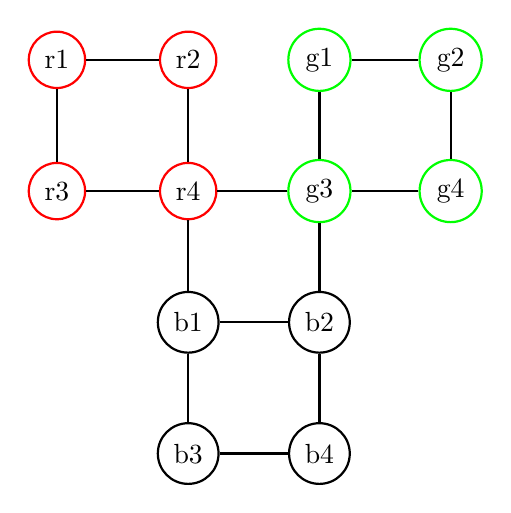
\begin{tikzpicture}\node[shape=circle,draw=red,align=center,line width=0.8pt] (0) at (2.5,13.333333333333334) {r1};
\node[shape=circle,draw=red,align=center,line width=0.8pt] (1) at (2.5,11.666666666666666) {r3};
\node[shape=circle,draw=red,align=center,line width=0.8pt] (2) at (4.166666666666667,11.666666666666666) {r4};
\node[shape=circle,draw=red,align=center,line width=0.8pt] (3) at (4.166666666666667,13.333333333333334) {r2};
\node[shape=circle,draw=green,align=center,line width=0.8pt] (4) at (5.833333333333333,11.666666666666666) {g3};
\node[shape=circle,draw=green,align=center,line width=0.8pt] (5) at (5.833333333333333,13.333333333333334) {g1};
\node[shape=circle,draw=green,align=center,line width=0.8pt] (6) at (7.5,13.333333333333334) {g2};
\node[shape=circle,draw=green,align=center,line width=0.8pt] (7) at (7.5,11.666666666666666) {g4};
\node[shape=circle,draw=black,align=center,line width=0.8pt] (8) at (4.166666666666667,10.0) {b1};
\node[shape=circle,draw=black,align=center,line width=0.8pt] (9) at (5.833333333333333,10.0) {b2};
\node[shape=circle,draw=black,align=center,line width=0.8pt] (10) at (5.833333333333333,8.333333333333334) {b4};
\node[shape=circle,draw=black,align=center,line width=0.8pt] (11) at (4.166666666666667,8.333333333333334) {b3};

\path [-,draw=black,line width=0.8pt] (0) edge node {} (3);
\path [-,draw=black,line width=0.8pt] (3) edge node {} (2);
\path [-,draw=black,line width=0.8pt] (2) edge node {} (1);
\path [-,draw=black,line width=0.8pt] (1) edge node {} (0);
\path [-,draw=black,line width=0.8pt] (5) edge node {} (6);
\path [-,draw=black,line width=0.8pt] (6) edge node {} (7);
\path [-,draw=black,line width=0.8pt] (7) edge node {} (4);
\path [-,draw=black,line width=0.8pt] (4) edge node {} (5);
\path [-,draw=black,line width=0.8pt] (8) edge node {} (9);
\path [-,draw=black,line width=0.8pt] (9) edge node {} (10);
\path [-,draw=black,line width=0.8pt] (10) edge node {} (11);
\path [-,draw=black,line width=0.8pt] (11) edge node {} (8);
\path [-,draw=black,line width=0.8pt] (4) edge node {} (9);
\path [-,draw=black,line width=0.8pt] (2) edge node {} (4);
\path [-,draw=black,line width=0.8pt] (2) edge node {} (8);
\end{tikzpicture}
\end{document}